\documentclass[xcolor=dvipsnames]{beamer}

\usepackage{graphicx,subfigure,url,pdfpages}

% example themes
\usetheme{Frankfurt}
\usecolortheme{owl}
\usecolortheme{rose}
\definecolor{myRed}{RGB}{180,11,11}
\definecolor{myWhite}{RGB}{170,170,170}
\setbeamercolor{title}{fg=myRed}
\setbeamercolor{frametitle}{fg=myRed}
\setbeamercolor{structure}{fg=myRed}
\setbeamercolor{normal text}{fg=myWhite}
% remove navigation symbols
\setbeamertemplate{navigation symbols}{}

\newcommand{\e}[1]{\times 10^{#1}}
\newcommand{\disp}{\textit{Disp }}
\title{DISP}
\author{Sreela}

\begin{document}

% \frame[plain]{\titlepage}

% \begin{frame}[plain]{Outline}
%   \tableofcontents
% \end{frame}

% \section{}
% \begin{frame}{MAError}
%     \begin{figure}[htbp]
%     \centering    
%     \subfigure{\includegraphics[width=0.48\linewidth]{TMVA_Disp_gamma/MAError_zen20}}
%     \subfigure{\includegraphics[width=0.48\linewidth]{TMVA_Disp_gamma/MAError_zen30}}
%     \subfigure{\includegraphics[width=0.48\linewidth]{TMVA_Disp_gamma/MAError_zen50}}
%     \subfigure{\includegraphics[width=0.48\linewidth]{TMVA_Disp_gamma/MAError_zen60}}
%     \caption{Calculated MA Error for zenith angles 20 (top-left), 30 (top-right), 50 (bottom-left) and 60 (bottom-right)}
%   \end{figure}
% \end{frame}
% {
%   \setbeamercolor{background canvas}{bg=}
%   \includepdf[pages=7]{dirReconstruction.pdf}
%   \includepdf[pages=8]{dirReconstruction.pdf}
% }

% \begin{frame}{MAError}
%     \begin{figure}[htbp]
%     \centering
%     \includegraphics[width=0.90\linewidth]{TMVA_Disp_gamma/MAError_impact_dist}
%     \caption{Calculated MA Err
%       or against impact distance in mirror plane}
%   \end{figure}
% \end{frame}
% \begin{frame}{Angular Resolution (Azimuth)}
%   \begin{figure}[htbp]
%     \centering
%     \subfigure{\includegraphics[width=.48\linewidth]{DevAz_reg}}
%     \subfigure{\includegraphics[width=.48\linewidth]{DevAz_disp}}
%     \caption{Deviation of reconstructed azimuth from simulated value for the standard method (left) and the disp method (right)}
%   \end{figure}

% \end{frame}
% \begin{frame}{Angular Resolution (Zenith)}
%   \begin{figure}[htbp]
%     \centering
%     \subfigure{\includegraphics[width=.48\linewidth]{DevZen_reg}}
%     \subfigure{\includegraphics[width=.48\linewidth]{DevZen_disp}}
%     \caption{Deviation of reconstructed zenith from simulated value for the standard method (left) and the disp method (right)}
%   \end{figure}

% \end{frame}
% \begin{frame}{Angular Resolution (Deg Sq)}
%   \begin{figure}[htbp]
%     \centering
%     \subfigure{\includegraphics[width=.48\linewidth]{DevSq_reg}}
%     \subfigure{\includegraphics[width=.48\linewidth]{DevSq_disp}}
%     \caption{Deviation of reconstructed angle (in deg sq) from simulated value for the standard method (left, 68\% containment at ${0.145^\circ}^2$) and the disp method (right, 68\% containment at ${0.045^\circ}^2$).}
%   \end{figure}
% \end{frame}

% \begin{frame}{68\% Containment vs Zenith}
% \begin{figure}[htbp]
%   \centering
%   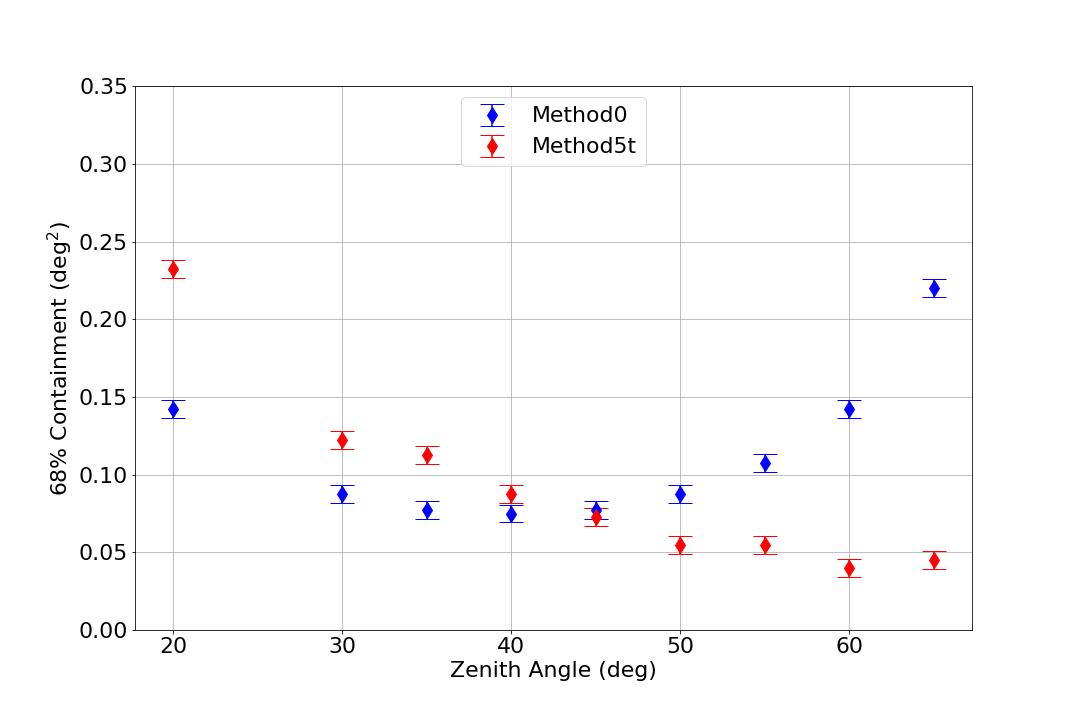
\includegraphics[width=.85\linewidth]{../python/disp_vs_reg}
%   \caption{68\% containment as a function of zenith angle for the regular method (blue) and the disp method (red)}
% \end{figure}
% \end{frame}

% \begin{frame}{68\% Containment vs Energy}
% \begin{figure}[htbp]
%   \centering
%   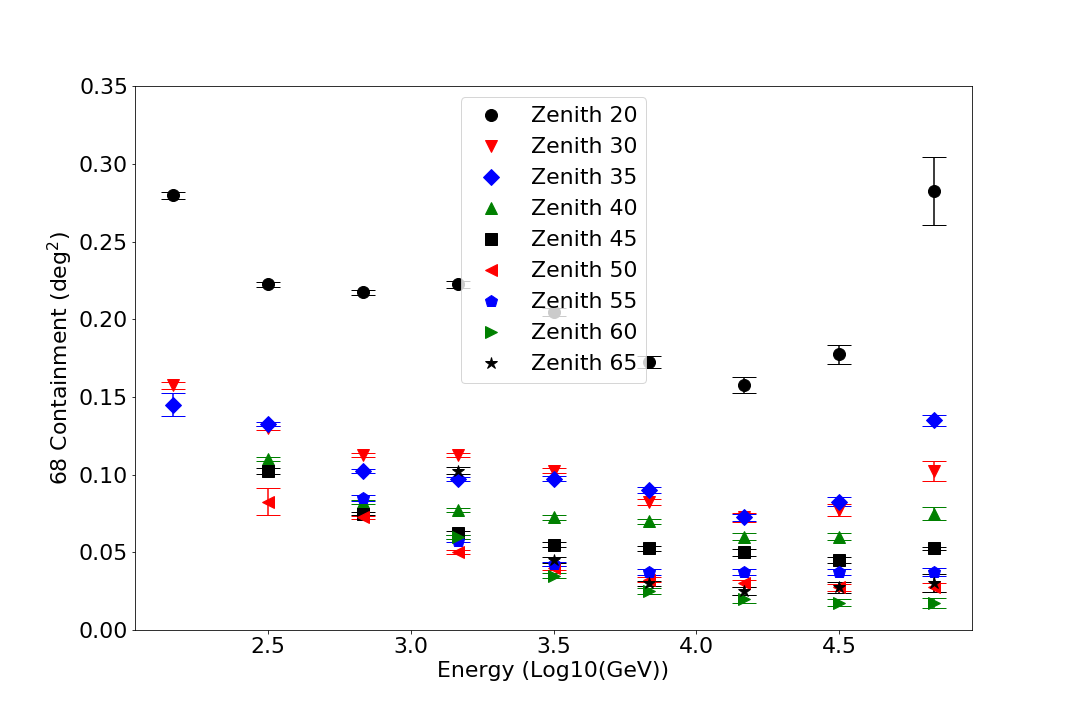
\includegraphics[width=.85\linewidth]{../python/disp_vs_energy}
%   \caption{68\% containment as a function of energy range}
% \end{figure}
% \end{frame}

% \begin{frame}{68\% Containment vs Energy}
%   \begin{figure}[htbp]
%     \centering
%     \subfigure{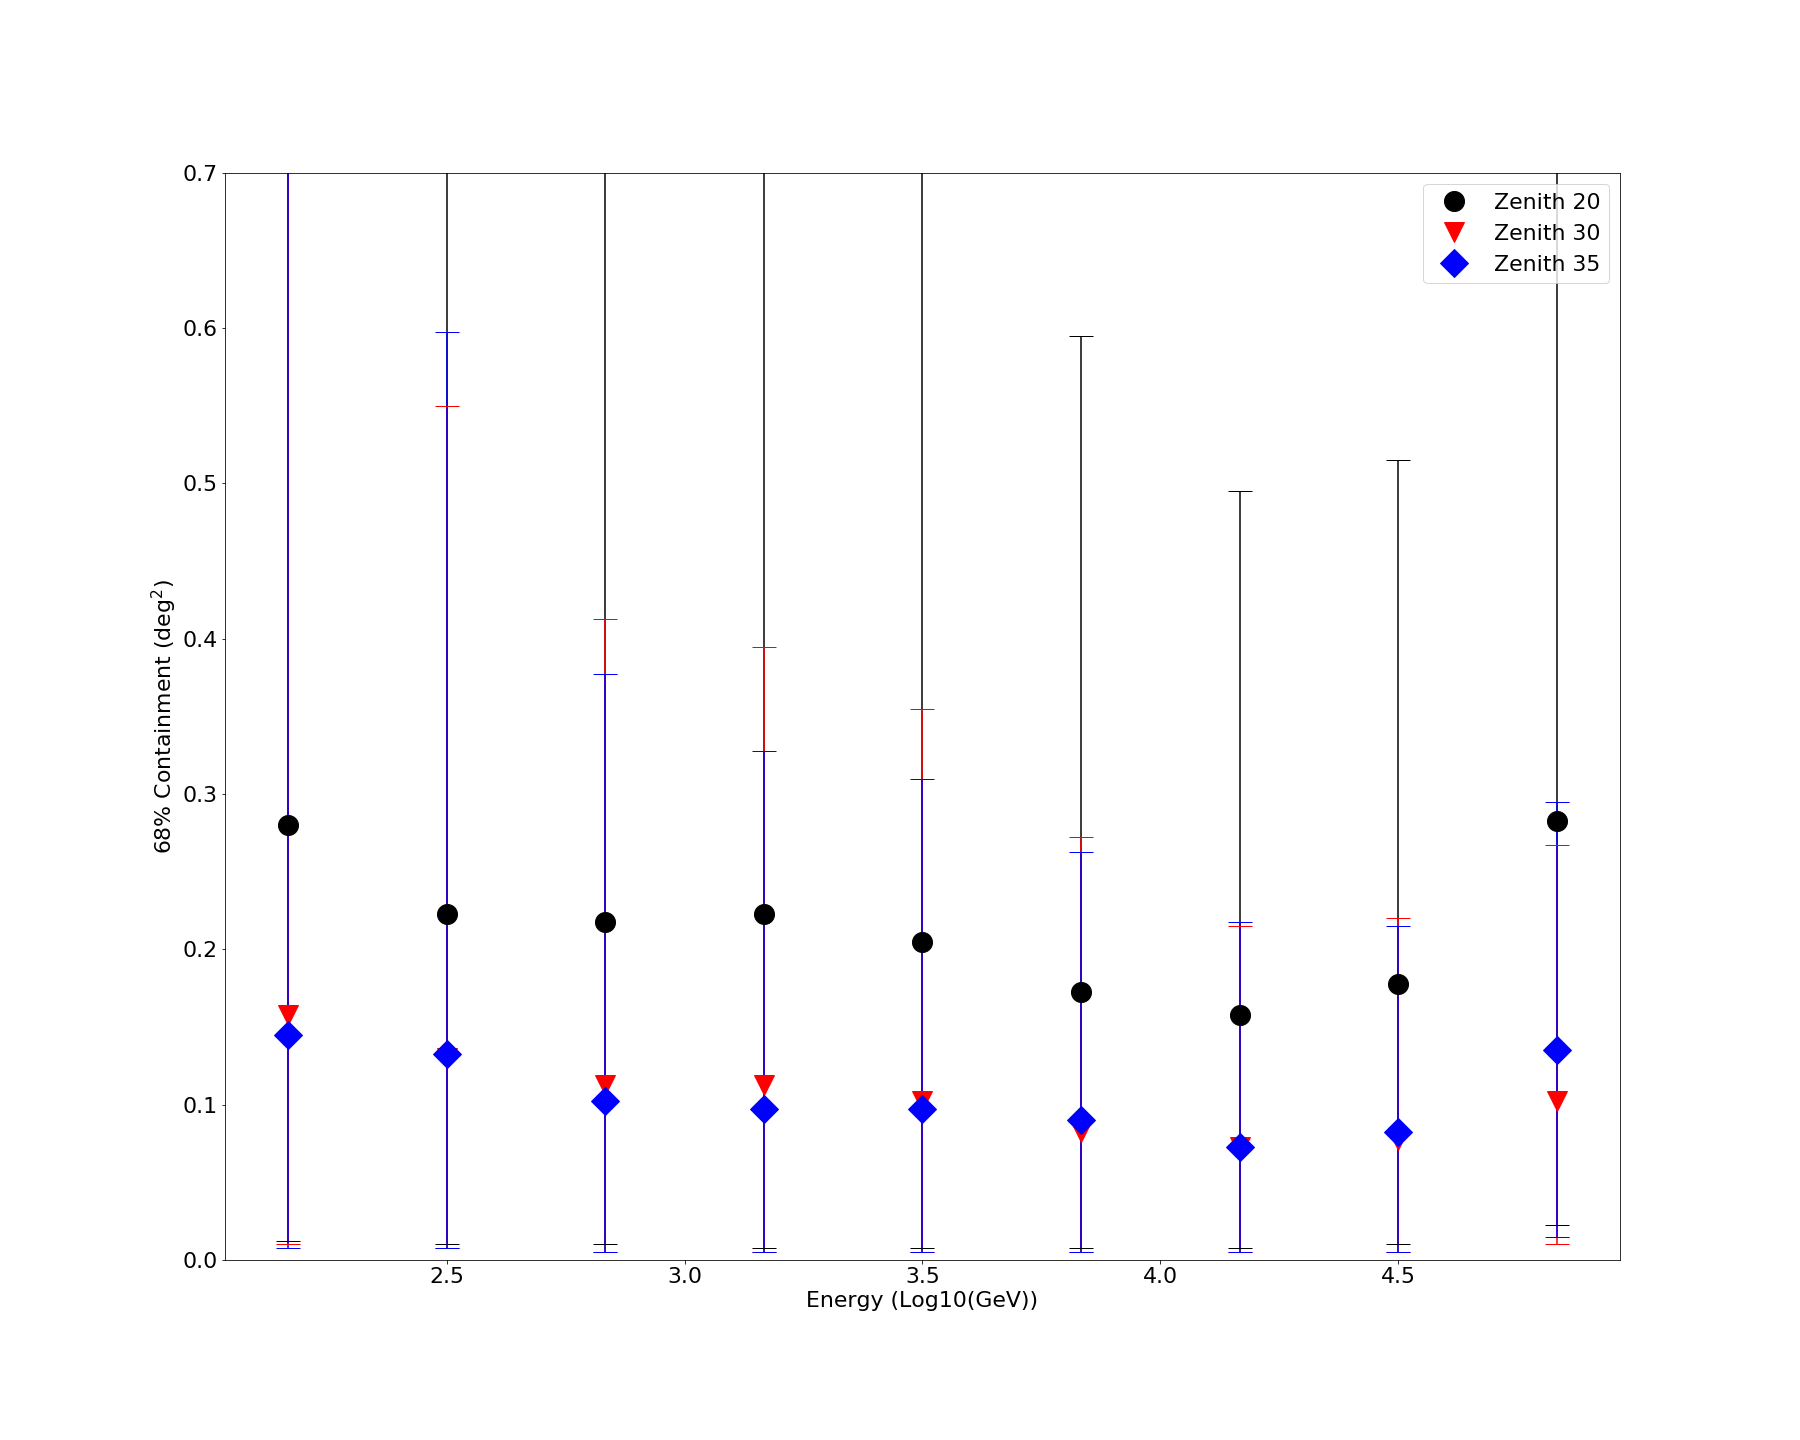
\includegraphics[width=.32\linewidth]{../python/disp_vs_energy_SZA}}
%     \subfigure{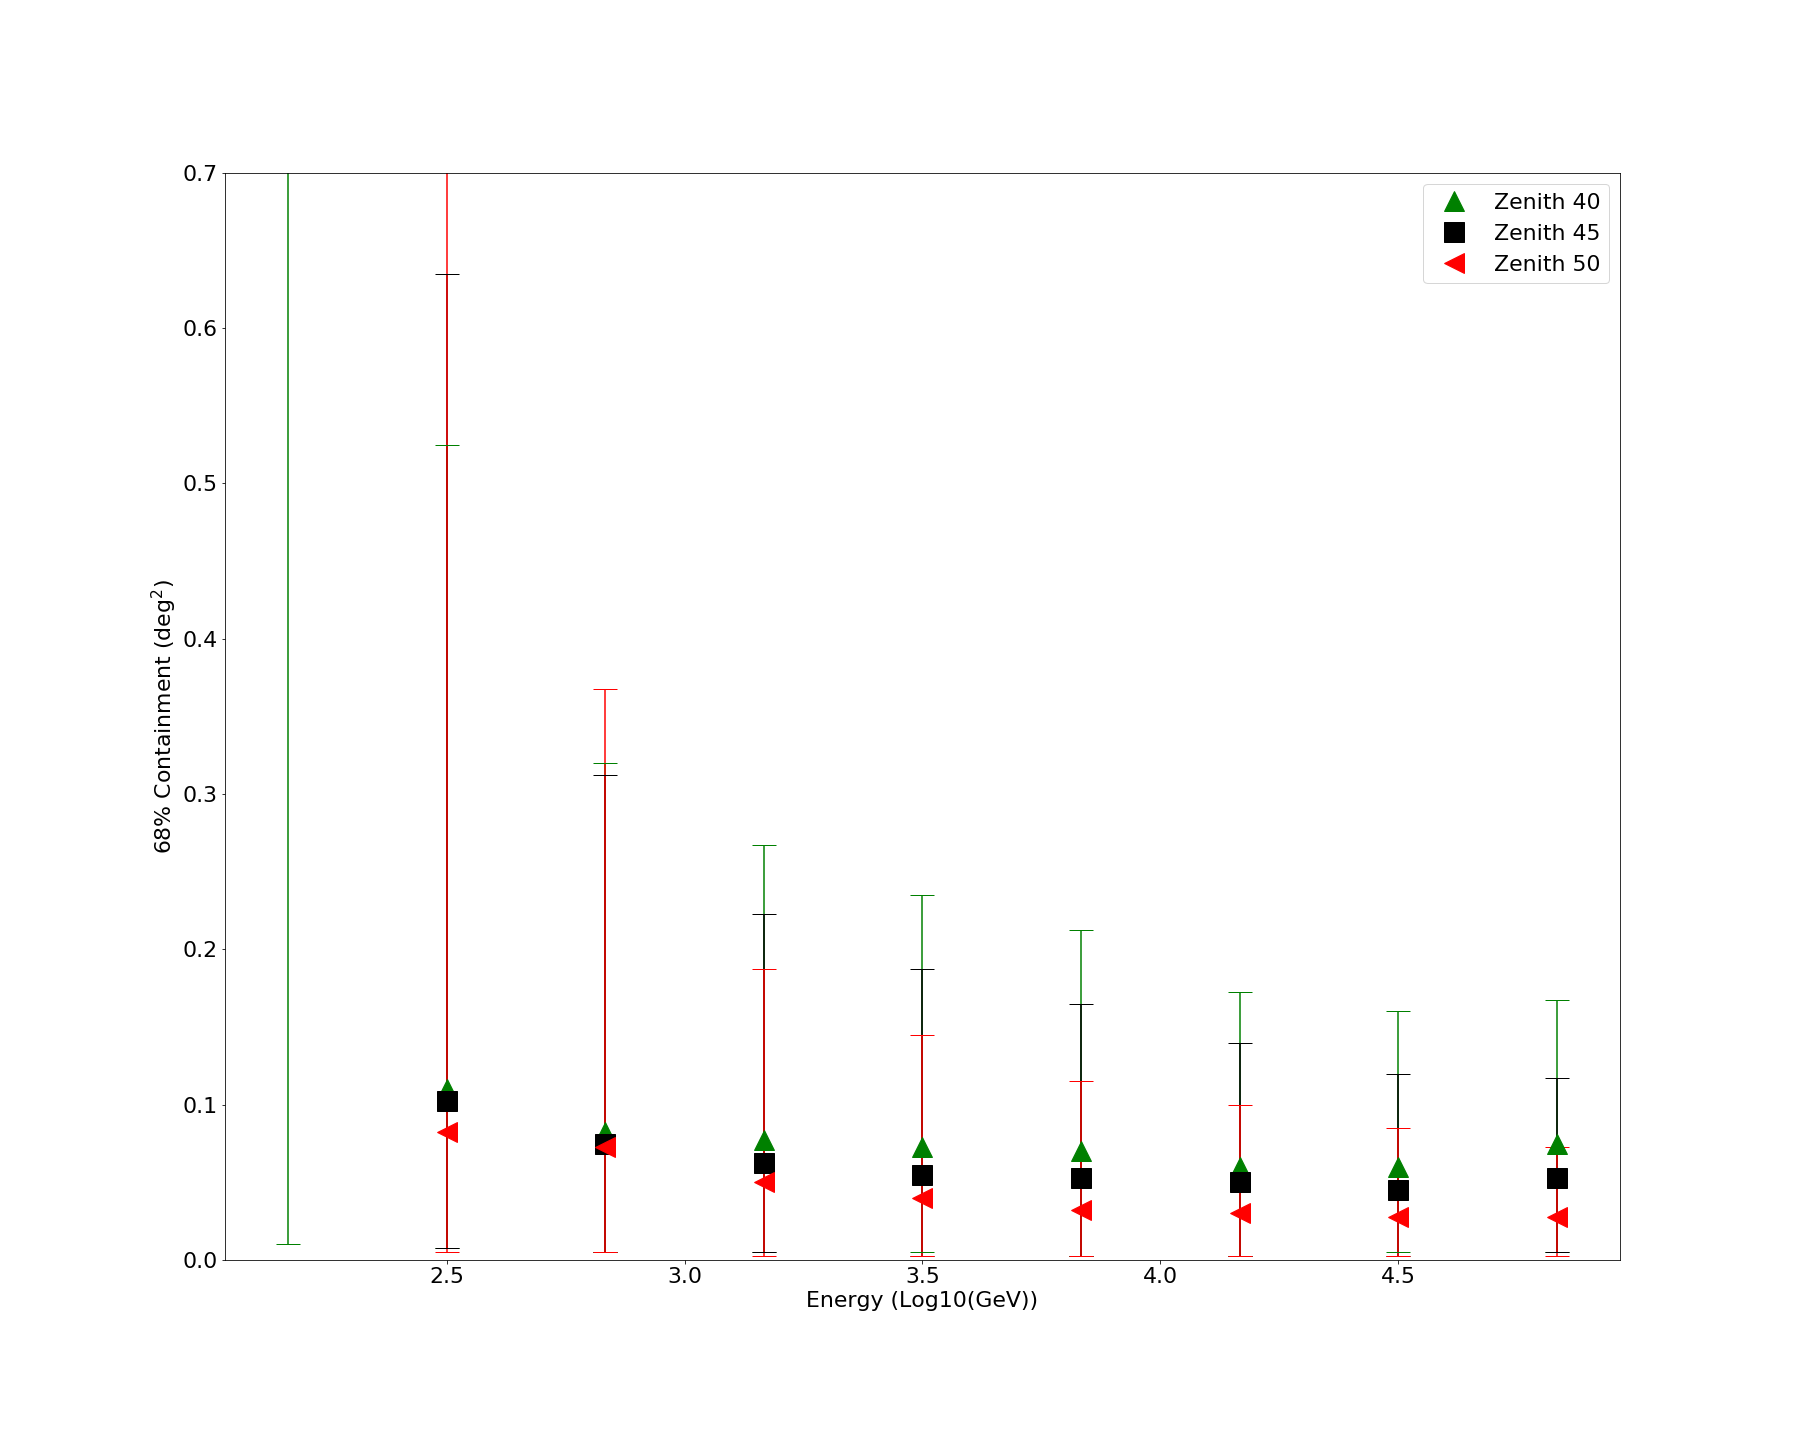
\includegraphics[width=.32\linewidth]{../python/disp_vs_energy_MZA}}
%     \subfigure{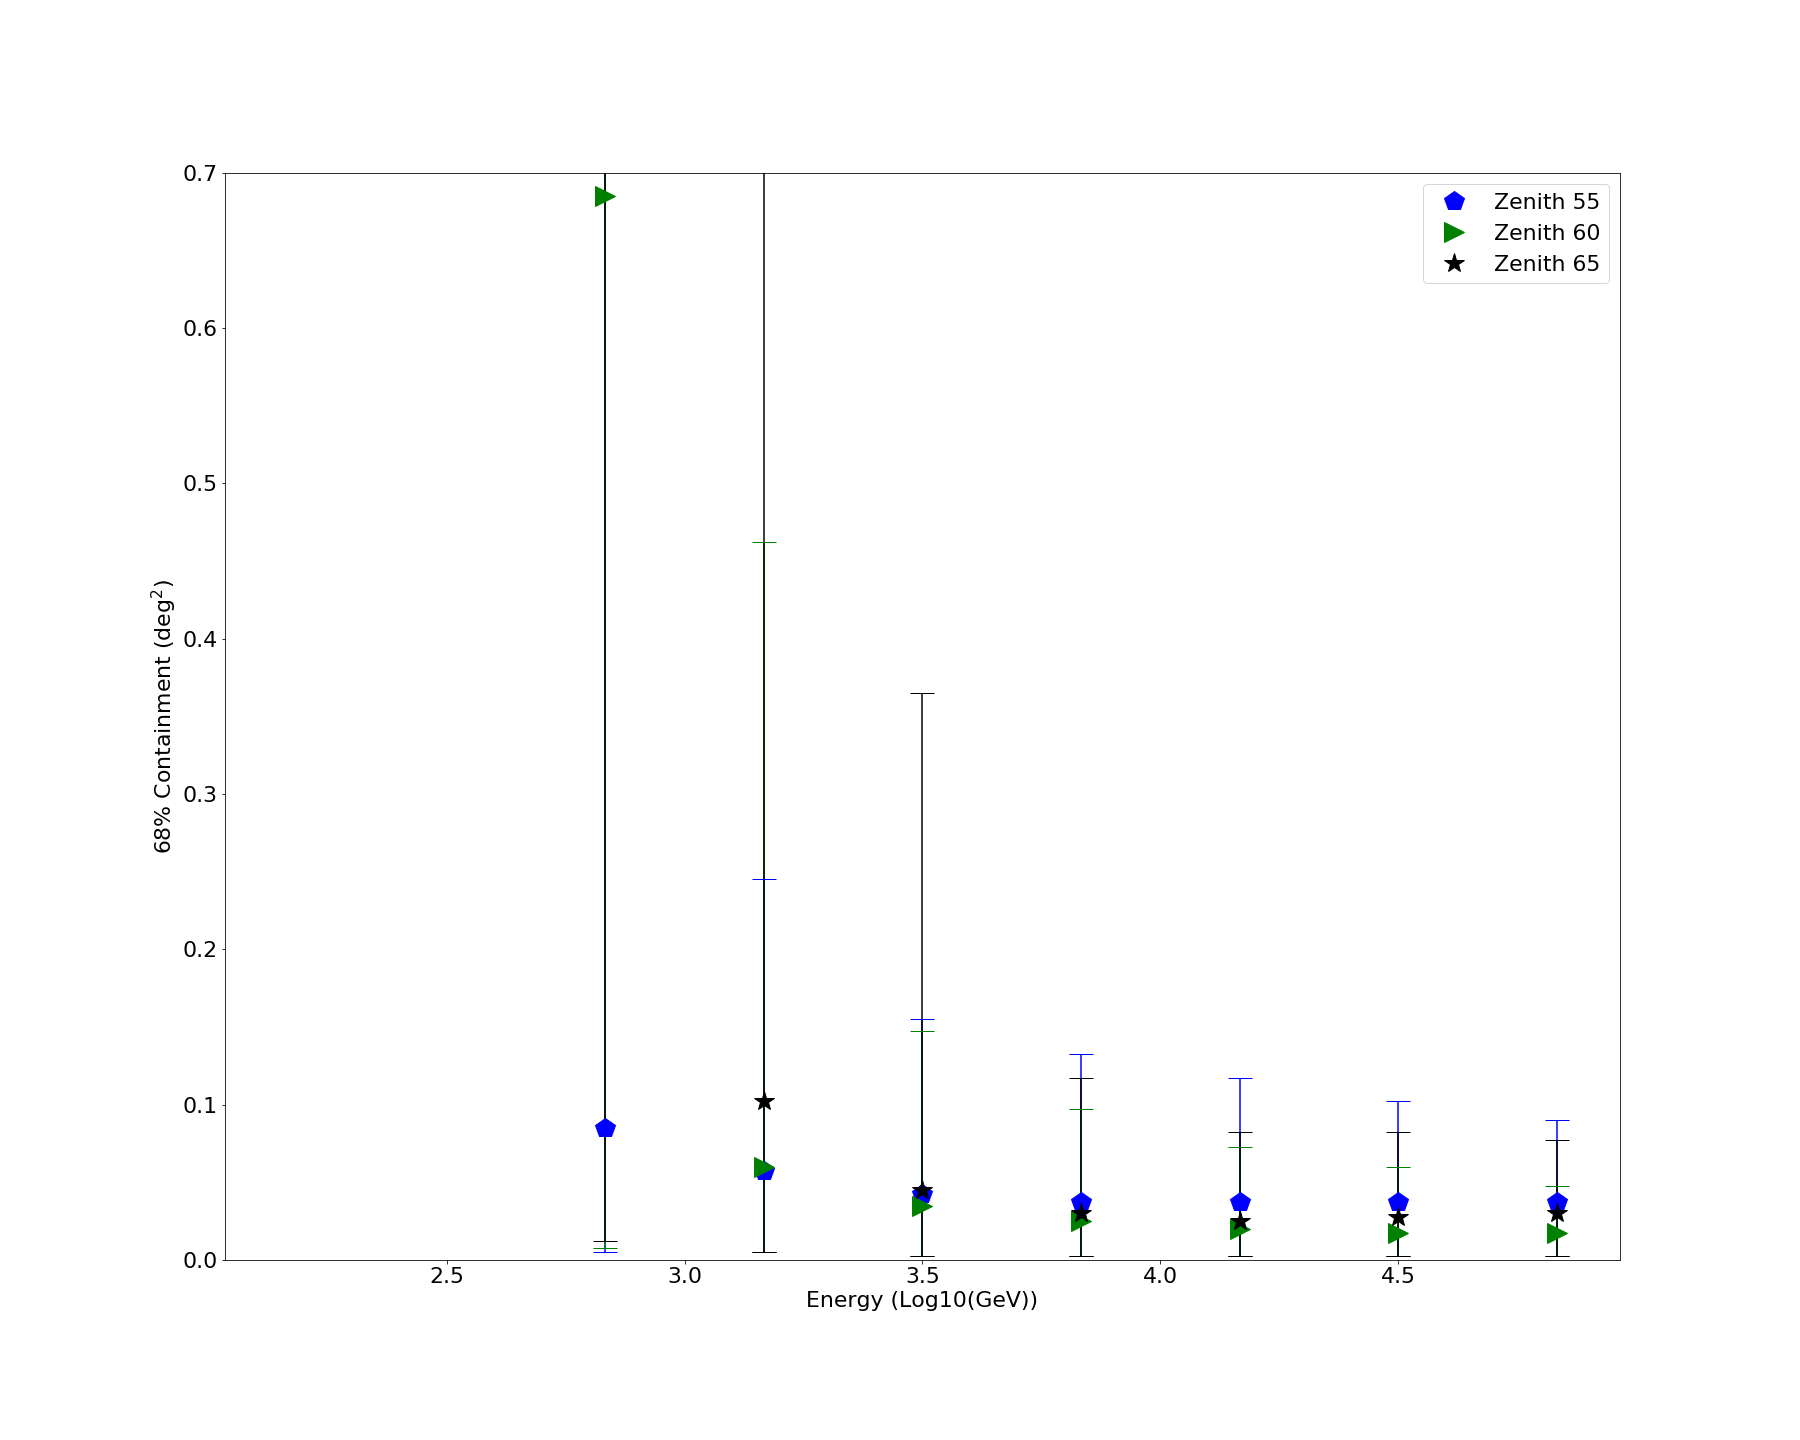
\includegraphics[width=.32\linewidth]{../python/disp_vs_energy_LZA}}
%     \caption{68\% containment as a function of energy range for the simulated zenith angle}
%   \end{figure}
% \end{frame}

% \begin{frame}{68\% Containment vs Energy and Zenith}
% \begin{figure}[htbp]
%   \centering
%   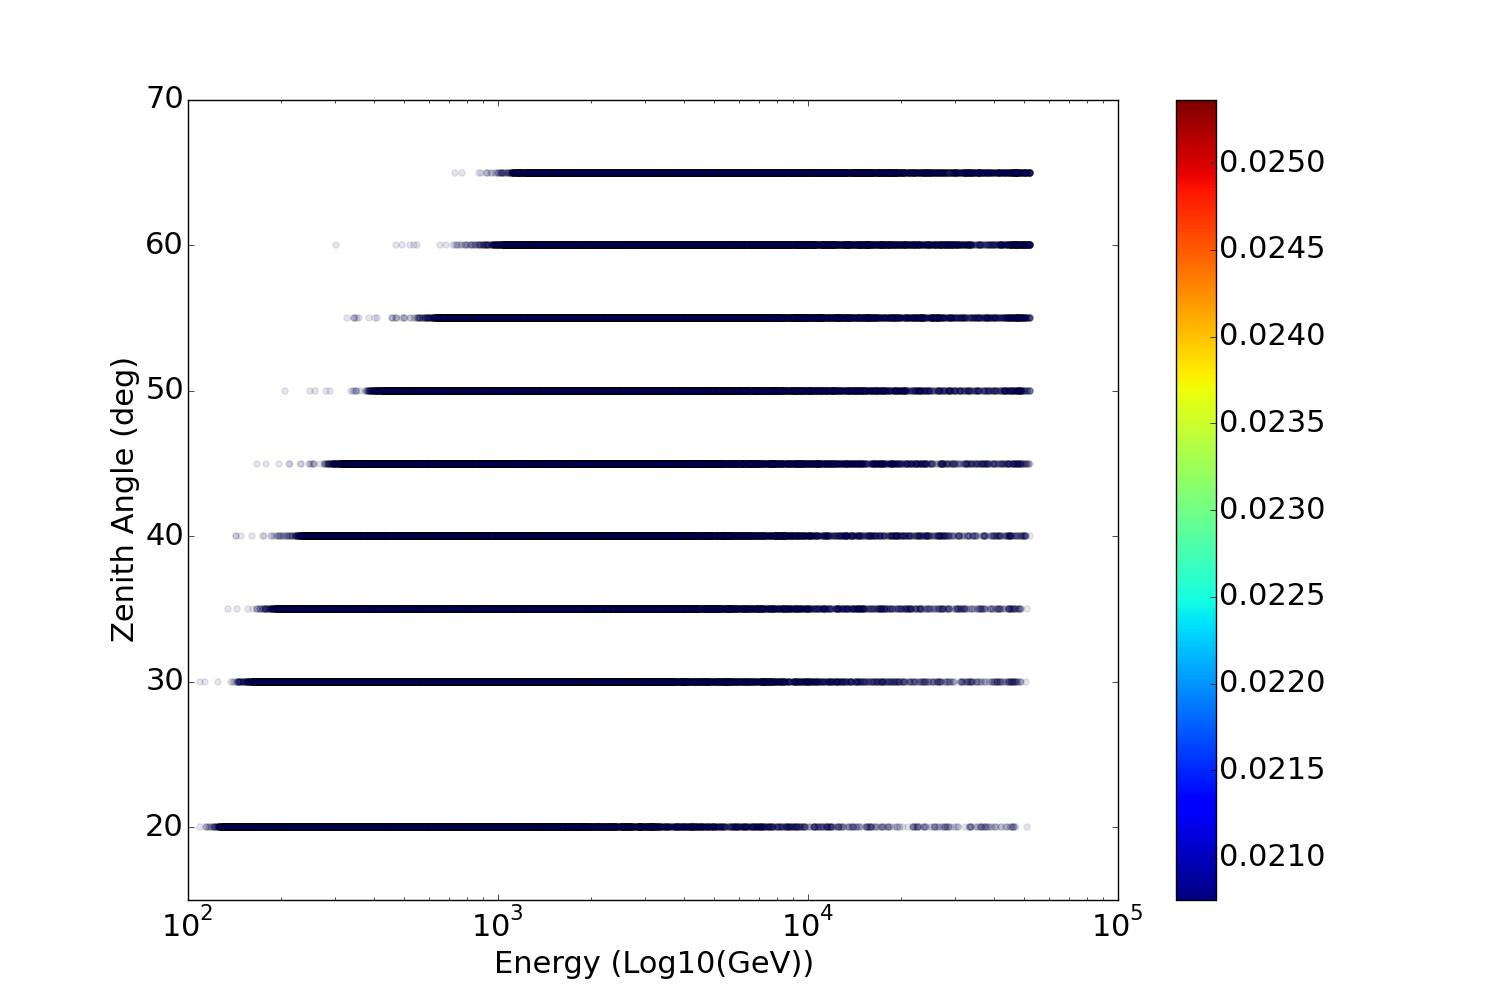
\includegraphics[width=.85\linewidth]{../python/energy_zenith_dev}
%   \caption{68\% containment distribution as a function of energy range and zenith}
% \end{figure}
% \end{frame}

% \begin{frame}{68\% Containment for Data Files\\ (Crab horizon-to-horizon 2018, 2019)}
% \begin{figure}[htbp]
%   \centering
%     \subfigure{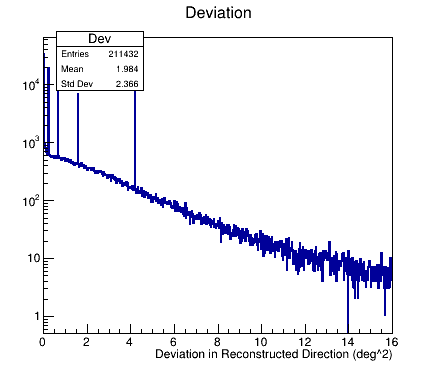
\includegraphics[width=.26\linewidth]{../python/reg_SZA_Dev}}
%     \subfigure{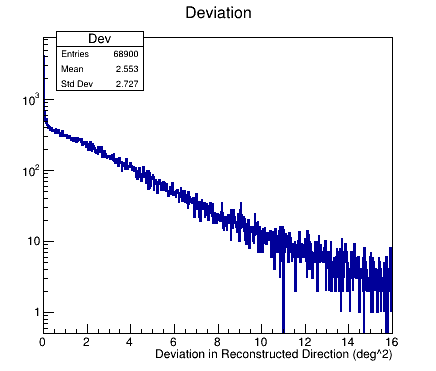
\includegraphics[width=.26\linewidth]{../python/reg_MZA_Dev}}
%     \subfigure{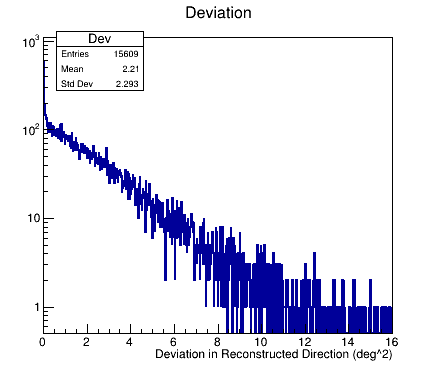
\includegraphics[width=.26\linewidth]{../python/reg_LZA_Dev}}
%     \subfigure{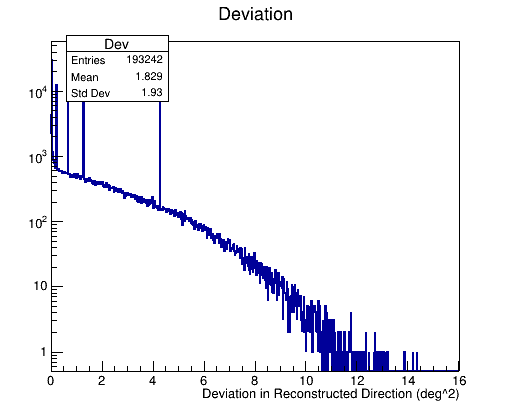
\includegraphics[width=.26\linewidth]{../python/newdisp_SZA_Dev}}
%     \subfigure{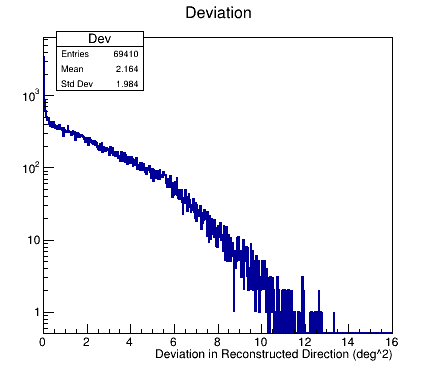
\includegraphics[width=.26\linewidth]{../python/newdisp_MZA_Dev}}
%     \subfigure{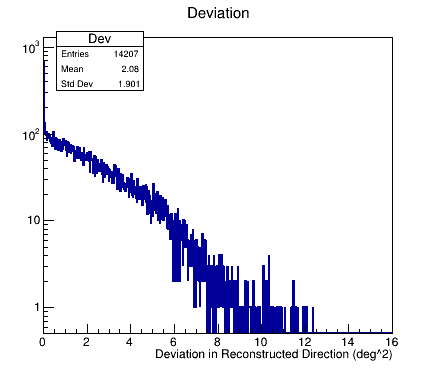
\includegraphics[width=.26\linewidth]{../python/newdisp_LZA_Dev}}
%     \caption{68\% containment for crab runs, Method0 (top) (\(0^\circ\)-\(30^\circ\), \(30^\circ\)-\(55^\circ\), \(55^\circ\)-\(90^\circ\)) (2.53, 2.98, 2.57), Method5t (bottom) (2.41, 2.73, 2.58)}
% \end{figure}
% \end{frame}

% \begin{frame}{Crab Spectral Index}
%   \begin{figure}[htbp]
%     \centering
%     \includegraphics[width=.92\linewidth]{Crab_C2C/Index_compare}
%     \caption{Spectral Index fit values using the two direction reconstruction methods}
%     \label{"CrabIndex"}
%   \end{figure}
% \end{frame}
% \begin{frame}{Crab Spectral Index}
%   \begin{figure}[htbp]
%     \centering
%     \includegraphics[width=.92\linewidth]{Crab_C2C/Index_zoom_reg}
%     \caption{Spectral Index fit values using the regular direction reconstruction method}
%     \label{"CrabIndex_reg"}
%   \end{figure}
% \end{frame}
% \begin{frame}{Crab Spectral Index}
%   \begin{figure}[htbp]
%     \centering
%     \includegraphics[width=.92\linewidth]{Crab_C2C/Index_zoom_disp}
%     \caption{Spectral Index fit values using the disp direction reconstruction method}
%     \label{"CrabIndex_disp"}
%   \end{figure}
% \end{frame}

% \begin{frame}{Crab Spectral Index}
% \begin{table}[H]
% \begin{center}
% \resizebox{0.8\textwidth}{!}{
%   \begin{tabular}{ l r r r }
% \hline
% Method & Value & Uncertainty & $\chi^2/d.o.f.$\\
% \hline\hline
%   reg horizontal line fit              &$    2.601 $&$   0.25  $&$   1.42  $\\
%   reg combined spectrum                &$    2.566 $&$   0.02  $&$   1.36  $\\
%   reg best fit line                    &Slope= 0.005 &$\pm$$ 0.003 $&$   1.340 $\\
%   disp horizontal line fit             &$    2.612 $&$   0.31  $&$   1.18  $\\
%   disp combined spectrum               &$    2.502 $&$   0.02  $&$   1.19  $\\
%   disp best fit line                   &Slope= 0.010 &$\pm$$ 0.003 $&$   0.941 $\\\hline
%   \end{tabular}}
  
% \caption{Spectral Index ($\Gamma$) fit values using the two methods using a weighted average (horizontal line fit), analyzing the entire set of runs 
% together (combined spectrum), and using a best fit line with non-zero slope.\label{table:index_values}. }
% \end{center}
% \end{table}
% \end{frame}

% \begin{frame}{Crab Integral Flux}
%   \begin{figure}[htbp]
%     \centering
%     \includegraphics[width=.92\linewidth]{Crab_C2C/Intf_compare}
%     \caption{Integral flux (from fit) above 2.239TeV, using the two direction reconstruction methods}
%     \label{"CrabIntf"}
%   \end{figure}
% \end{frame}

% \begin{frame}{Crab Integral Flux}
%   \begin{figure}[htbp]
%     \centering
%     \includegraphics[width=.92\linewidth]{Crab_C2C/Intf_zoom_reg}
%     \caption{Integral flux (from fit) above 2.239TeV, using the regular direction reconstruction method}
%     \label{"CrabIntf_reg"}
%   \end{figure}
% \end{frame}

% \begin{frame}{Crab Integral Flux}
%   \begin{figure}[htbp]
%     \centering
%     \includegraphics[width=.92\linewidth]{Crab_C2C/Intf_zoom_disp}
%     \caption{Integral flux (from fit) above 2.239TeV, using the disp direction reconstruction method}
%     \label{"CrabIntf_disp"}
%   \end{figure}
% \end{frame}

% \begin{frame}{Crab Integral Flux}
%   \begin{figure}[htbp]
%     \centering
%     \includegraphics[width=.92\linewidth]{Compare_disp/Intf_compare}
%     \caption{Integral flux (from fit) above 2.239TeV, using the old and new disp direction reconstruction methods}
%     \label{"CrabIntf"}
%   \end{figure}
% \end{frame}

% \begin{frame}{Crab Integral Flux}
%   \begin{figure}[htbp]
%     \centering
%     \includegraphics[width=.92\linewidth]{Compare_disp/Intf_zoom_reg}
%     \caption{Integral flux (from fit) above 2.239TeV, using the old disp direction reconstruction method}
%     \label{"CrabIntf_reg"}
%   \end{figure}
% \end{frame}

% \begin{frame}{Crab Integral Flux}
%   \begin{figure}[htbp]
%     \centering
%     \includegraphics[width=.92\linewidth]{Compare_disp/Intf_zoom_disp}
%     \caption{Integral flux (from fit) above 2.239TeV, using the new disp direction reconstruction method}
%     \label{"CrabIntf_disp"}
%   \end{figure}
% \end{frame}

% \begin{frame}{Crab Integral Flux}
% \begin{table}[H]
% \begin{center}
% \resizebox{0.8\textwidth}{!}{
% \begin{tabular}{ l r r r }
% \hline
% Method & \shortstack{Value \\$(10^{7}$m$^{2}$s$^{1})^{-1}$} & \shortstack{Uncertainty \\$(10^{8}$m$^{2}$s$^{1})^{-1}$} & $\chi^2/d.o.f.$\\
% \hline\hline
%   reg horizontal line fit              &$    0.408 $&$   1.74  $&$   1.42  $\\
%   reg combined spectrum                &$    0.461 $&$   0.16  $&$   1.81  $\\
%   reg best fit line                    &Slope= -0.002 &$\pm$$ 0.02 $&$   1.30  $\\
%   disp horizontal line fit             &$    0.261 $&$   1.46  $&$   2.01  $\\
%   disp combined spectrum               &$    0.350 $&$   0.15  $&$   3.73  $\\
%   disp best fit line                   &Slope= -0.004 &$\pm$$ 0.02 $&$   1.40  $\\
%   \hline
% \end{tabular}}
% \caption{Integral Flux (from fit) above 2.239TeV using the two methods using a weighted average (horizontal line fit), analyzing the entire set of runs 
% together (combined spectrum), and using a best fit line with non-zero slope. \label{table:intf_values}}
% \end{center}
% \end{table}
% \end{frame}


% \begin{frame}{68\% Containment for Data Files (Crab coast to coast 2018-2019)}
% \begin{figure}[htbp]
%   \centering
%     \subfigure{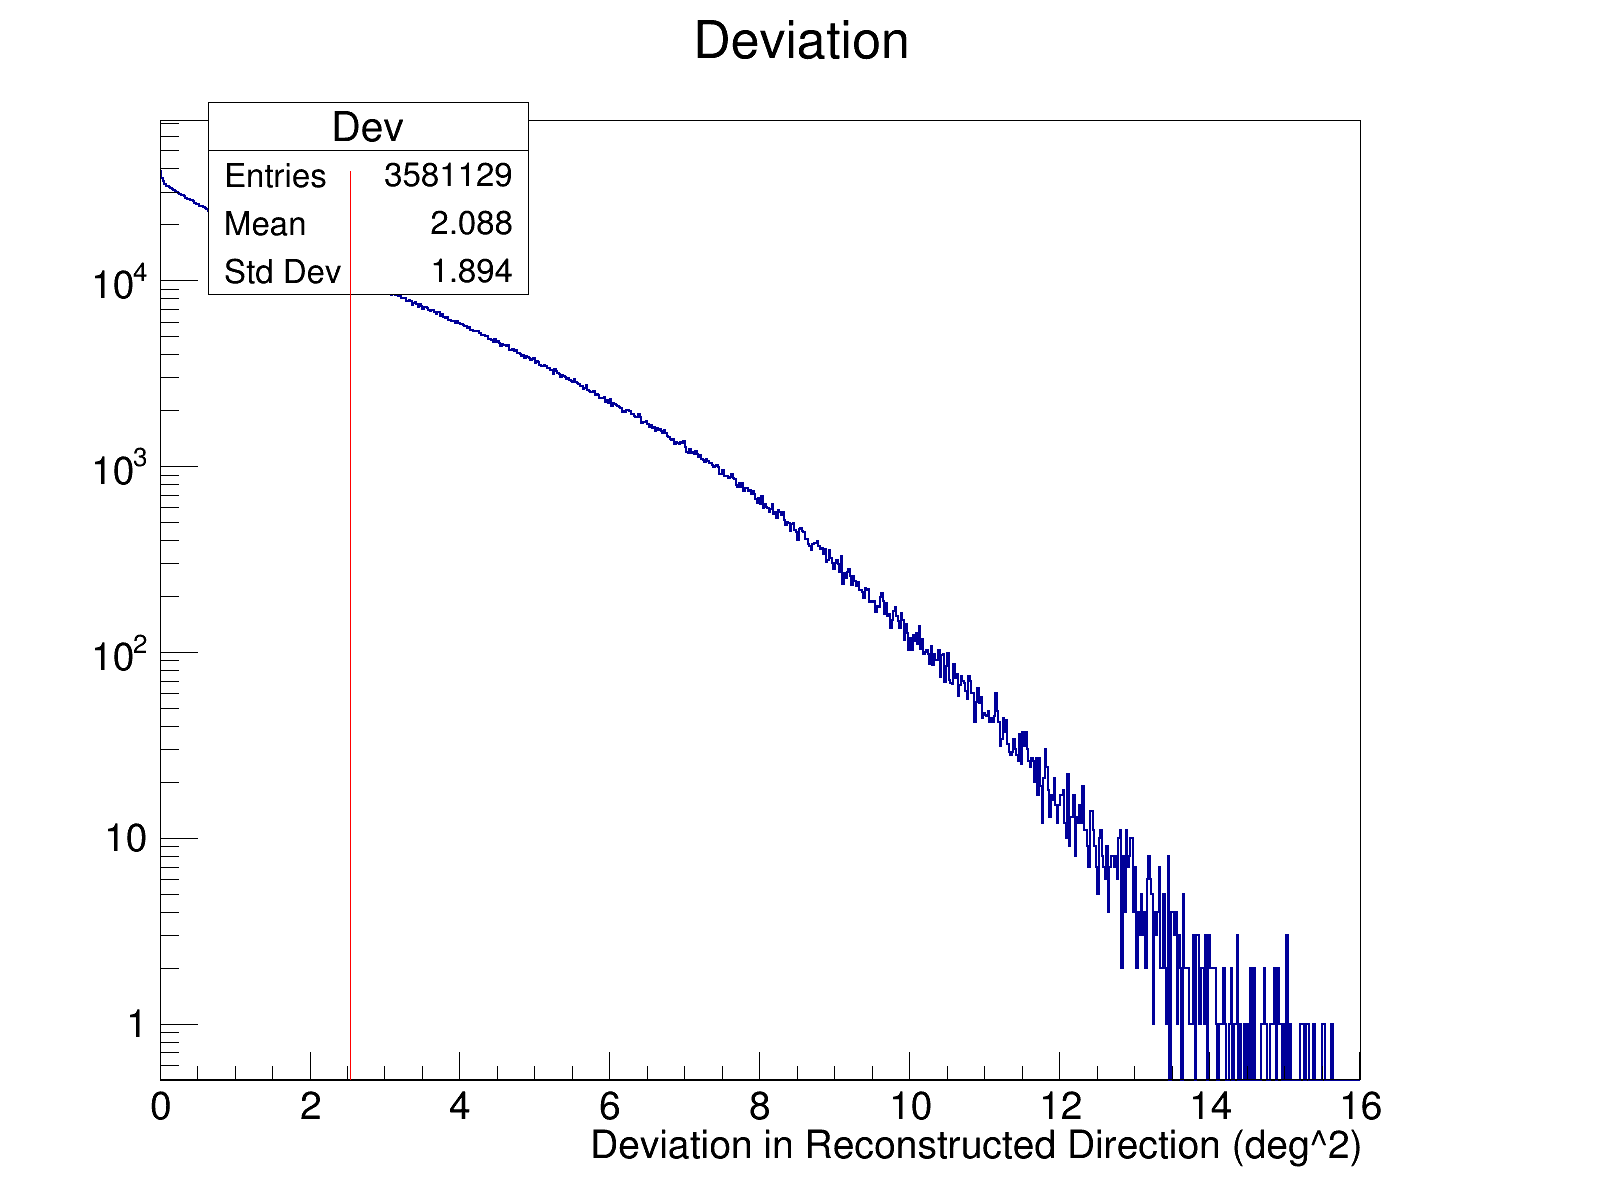
\includegraphics[width=.26\linewidth]{../python/newdisp_both_SZA}}
%     \subfigure{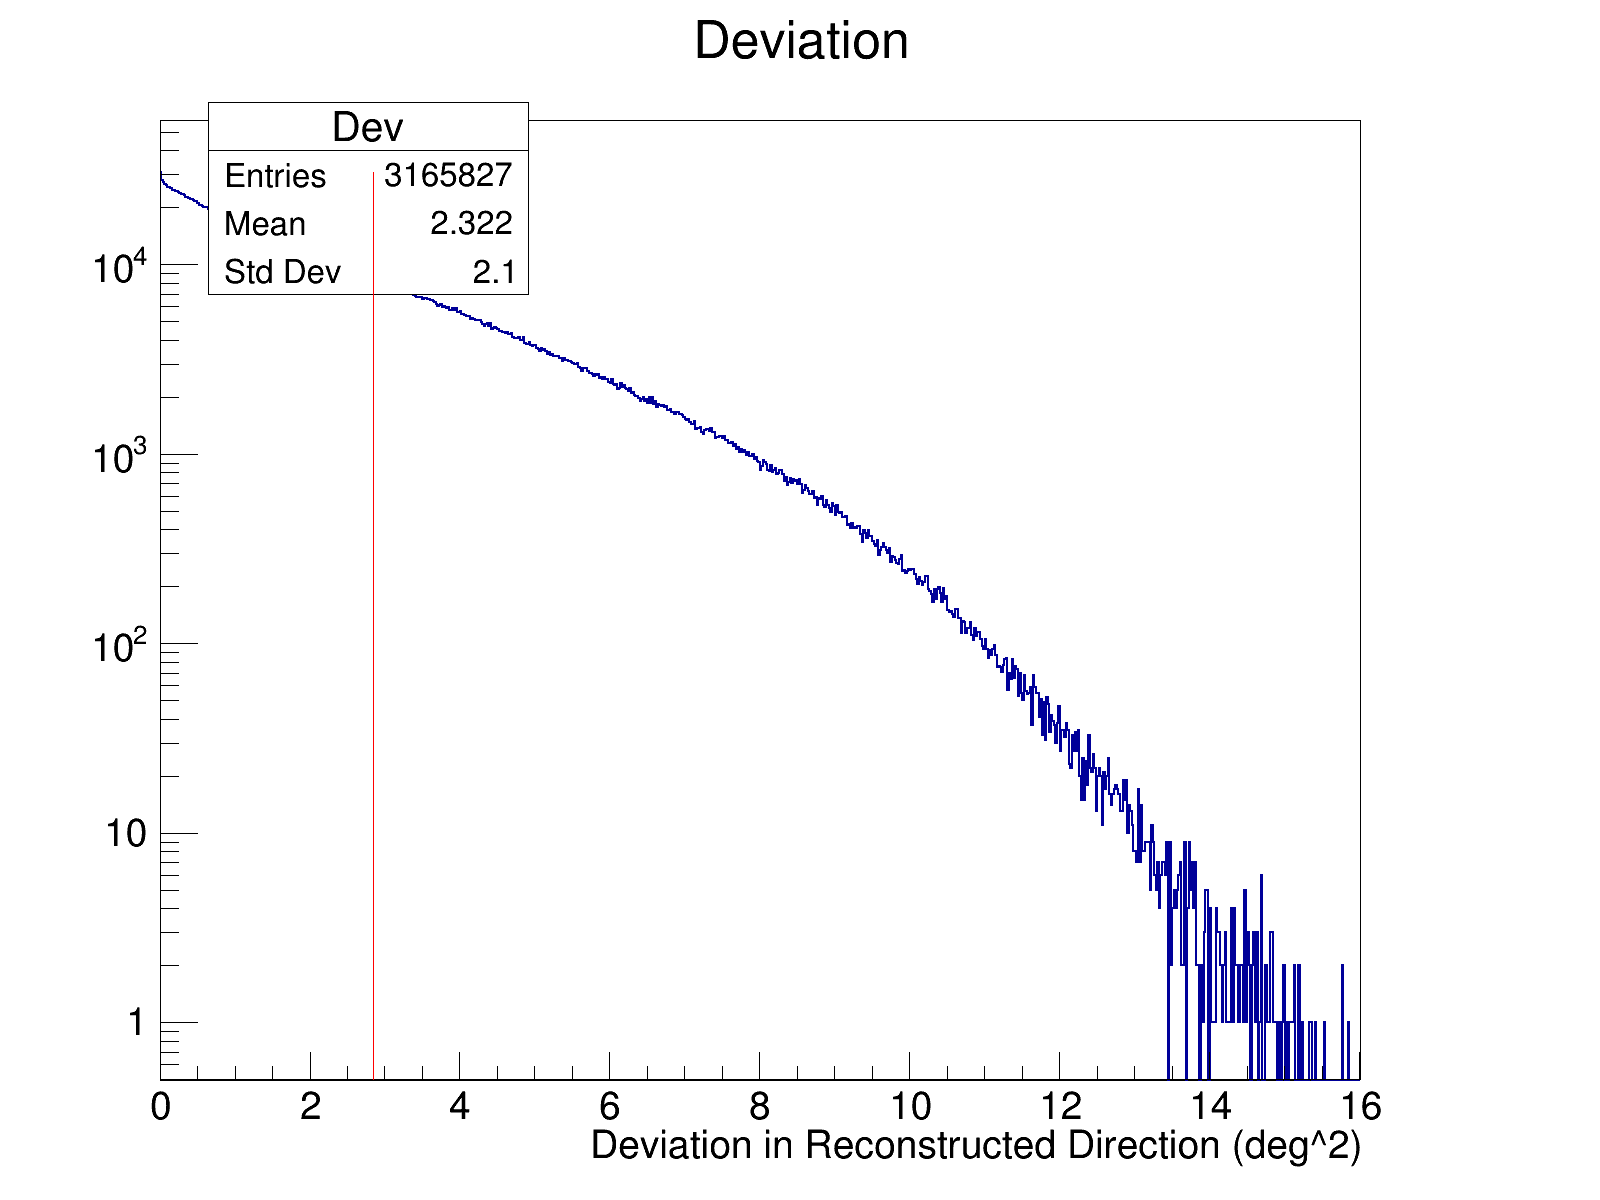
\includegraphics[width=.26\linewidth]{../python/newdisp_both_MZA}}
%     \subfigure{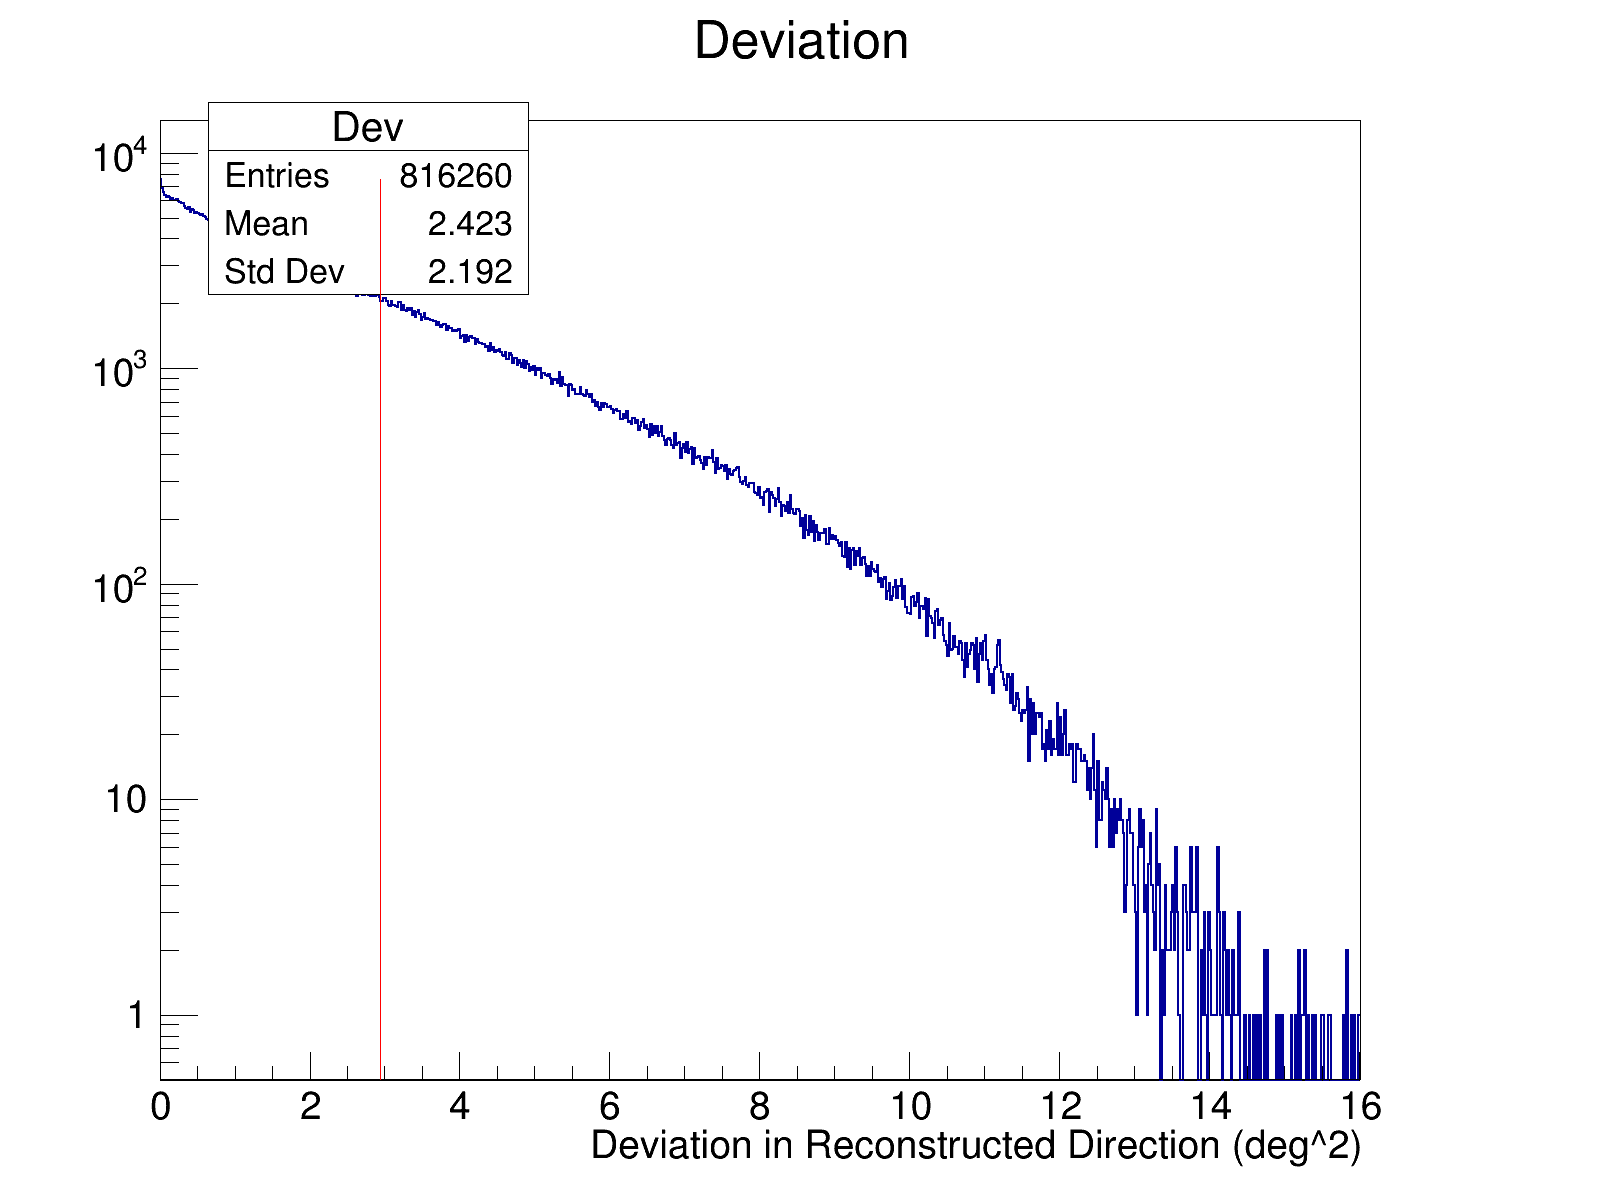
\includegraphics[width=.26\linewidth]{../python/newdisp_both_LZA}}
%   \caption{68\% containment for crab runs 2018-2019, Method5t (bottom) (2.54, 2.84, 2.94)}
% \end{figure}
% \end{frame}

\begin{frame}{68\% Containment for Simulation Files (Disp table at noise=250MHz)}
  \begin{figure}[H]
  \centering
    \subfigure{\includegraphics[width=0.48\linewidth]{../python/sims_olddisp/zenall_val}}  
    \subfigure{\includegraphics[width=0.48\linewidth]{../python/sims_250disp/zenall_val}}
  \caption{Reconstruction of simulation files using the standard \disp tables (left) and the toy \disp tables ($\sim3.9\e6$ events all at noise $= 250$ MHz)}
\end{figure}
\end{frame}
\begin{frame}{68\% Containment for Simulation Files (Disp table at noise=250MHz)}
  \begin{figure}[H]
  \centering
    \subfigure{\includegraphics[width=0.48\linewidth]{../python/sims_olddisp/zenall_ratio_thesis}}  
    \subfigure{\includegraphics[width=0.48\linewidth]{../python/sims_250disp/zenall_ratio_thesis}}
  \caption{Reconstruction of simulation files using the standard \disp tables (left) and the toy \disp tables ($\sim3.9\e6$ events all at noise $= 250$ MHz)}
\end{figure}
\end{frame}

\begin{frame}{68\% Containment for Simulation Files (Disp table at noise=450MHz)}
  \begin{figure}[H]
  \centering
    \subfigure{\includegraphics[width=0.48\linewidth]{../python/sims_olddisp/zenall_val}}  
    \subfigure{\includegraphics[width=0.48\linewidth]{../python/sims_450disp/zenall_val}}
  \caption{Reconstruction of simulation files using the standard \disp tables (left) and the toy \disp tables ($\sim 4.2\e6$ events all at noise $= 450$ MHz)}
\end{figure}
\end{frame}

\begin{frame}{68\% Containment for Simulation Files (Disp table at noise=450MHz)}
  \begin{figure}[H]
  \centering
    \subfigure{\includegraphics[width=0.48\linewidth]{../python/sims_olddisp/zenall_ratio_thesis}}  
    \subfigure{\includegraphics[width=0.48\linewidth]{../python/sims_450disp/zenall_ratio_thesis}}
  \caption{Reconstruction of simulation files using the standard \disp tables (left) and the toy \disp tables ($\sim 4.2\e6$ events all at noise $= 450$ MHz)}
\end{figure}
\end{frame}

\end{document}

%%% Local Variables:
%%% mode: latex
%%% TeX-master: t
%%% End:
